\documentclass[pdftex,12pt,a4paper,openany,fleqn]{article}

\usepackage[english]{babel}
\usepackage[utf8x]{inputenc}
\usepackage{appendix}
\usepackage{amsmath}
%\usepackage[textsize=footnotesize]{todonotes}
\usepackage[top=0.5in, text={6.8in,10.3in}]{geometry}
\usepackage{hyperref}
% usepackages not included in writelatex
\usepackage[dvips]{graphicx}
\usepackage[usenames,dvipsnames]{color}% colored fonts ("usenames" defines 68 colors  http://en.wikibooks.org/wiki/LaTeX/Colors)
\usepackage[sort&compress,numbers]{natbib} % bibliographic style (sorted numbers)
\usepackage{nameref}  % standard references (to chapter, page)
\usepackage{times}    % recommended fonts for pdflatex
\usepackage{mathpazo} % recommended fonts for pdflatex
\usepackage{courier}  % recommended fonts for pdflatex
\usepackage{helvet}   % recommended fonts for pdflatex
\usepackage{cmap}     % to produce searchable PDF
\usepackage{amsmath}
\usepackage{url} % quick-dirty replacement to "\tt"; use as "\path{}"; [obeyspaces] option to avoid unix-like no-space paths
\usepackage{microtype} % fixes typography, minimizing overbox etc. (that is, solves the \tt problem without \path{})
\usepackage{amsfonts}
\usepackage{amssymb}
\usepackage{amsthm}
\usepackage{multirow}  % fields that span multiple rows in tabular environment
\usepackage{setspace} % use as \begin{spacing}{0.8} to reduce linespacing to 80% 
\usepackage[margin=20pt,font=normal,labelfont=bf]{caption, subfig}  % caption and subfigure (composite figs) control 
\usepackage{authblk} % authors and \affil

\renewcommand\Authfont{\fontsize{12}{16}\selectfont}
\renewcommand\Affilfont{\fontsize{10}{12}\itshape}

\bibliographystyle{unsrt}
\linespread{1.5}

\renewcommand\floatpagefraction{.9} %page fraction with figures/tables 
\renewcommand\topfraction{.9}       %page fraction with figures/tables 
\renewcommand\bottomfraction{.9}    %page fraction with figures/tables 
\renewcommand\textfraction{.1}      %page fraction with text 
\setlength{\parskip}{2ex plus 0.5ex minus 0.2ex} % vertical space between paragraphs
\setlength{\parindent}{0ex} % no indentation for first line of each paragraph
\newcommand{\deriv}{\;\mathrm{d}}

\definecolor{blucol}{rgb}{0,0.4,0.7}
\newcommand{\blue}{\textcolor{blucol}}
\newcommand{\green}{\textcolor{green}}
\newcommand{\red}{\textcolor{red}}
\newcommand{\magenta}{\textcolor{magenta}}
\newcommand{\cyan}{\textcolor{cyan}}
\definecolor{orangecol}{rgb}{1,0.5,0}
\newcommand{\orange}{\textcolor{orangecol}}

%\setlength{\marginparwidth}{4.3cm} %for todonotes
\renewcommand\floatpagefraction{.8} %page fraction with figures/tables 
\renewcommand\topfraction{.8}       %page fraction with figures/tables 
\renewcommand\bottomfraction{.8}    %page fraction with figures/tables 
\renewcommand\textfraction{.2}      %page fraction with text 
\setcounter{totalnumber}{50}  % max figures per page
\setcounter{topnumber}{50}    % max figures per page
\setcounter{bottomnumber}{50} % max figures per page

\renewcommand*{\familydefault}{\sfdefault}
\title{Spectral signature of gene family trees}
\author[1]{Leonardo de Oliveira Martins\thanks{{\tt Leonardo.de-Oliveira-Martins@quadram.ac.uk}}}
\author[2,3]{Christophe Dessimoz\thanks{{\tt cdessimoz@unil.ch}}}
\affil[1]{Quadram Institute Biosciences, Norwich, NR4 7UQ, UK}
\affil[2]{UNIL}
\affil[3]{UCL}
\date{\vspace{-5ex}}
\begin{document}
\maketitle

\begin{abstract}
this is the abstract
\end{abstract}

%Christophe's comments: Finish drafting paragraphs that are in outline form.
%* In particular, check consistency of terms gene/sample and species/reference (stick to ‘gene’ and ‘reference’?)
%* Interpretation of fungi example. What does this tell us? (give an example of “gene shopping”?)
%Abstract
%--- nice to have ---
%* On empirical data, cluster (either using an automated method, or quadrants, or by hand), and try to reconstruct a consensus tree for each cluster vs. overall consensus tree.
%* Potential discussion point: discrete clusters or continuum? ILS and “isolated” HGT events, missing data, inference errors -> probably better modeled as a continuum -> interesting to see the extremes?

A fundamental unit in phylogenomic analysis is the gene (or genomic locus), and the most detailed evolutionary
history of a gene includes the duplication and loss events by which an ancestral locus gave rise to all
observed diversity of loci and genes --- the so-called gene family, of which a single copy gene is a particular case.
Each gene family will then be described by all the loci within a species connected through an common ancestor 
(i.e. inferred to be homologous to each other).
And their histories are expected to differ from one another due to the coalescent, duplications, losses, and
other biological events.
Therefore, even for the simplest case of single copy genes, we might still observe distinct patterns of their presence and
absence amongst species, and conflicting inferred phylogenies due to the coalescent, lateral transfers, and the very
inference process. 
The accumulation of large-scale phylogenomic data sets leads to new challenges of comparison and visualisation of
distinct gene families, as well as of detecting the influence of each genomic region into the overall phylogenomic
signals.
Many state-of-the-art phylogenetic methods take gene trees as input, and model the incongruence among them in
various ways, based on parametric and non-parametric assumptions \citep{astral, astrid}.
Many of these methods require the input gene trees to have at most one
representative from each species (e.g. by requiring the user to first run an orthology inference pipeline). 
This limitation is hard to circumvent since almost all tree distance measures (required to measure incongruence between
two trees) assume that the same leaves are present on both trees.

There has been several attempts at describing phylogenetic trees as vectors of features, suitable for statistical
comparison, such as \cite{Leigh2008, Leigh2011, Susko2006, Narechania2016, Nye2011, Yoshida2015, Lewitus2015,
Kendall2016, Colijn2018}. 
There are also a few methods that rely on pairwise tree distance matrices, which could then be projected into a new
coordinate system.

Unsupervised learning algorithms accept one of two forms of input: a design (also called feature) matrix $X$ of size
$n\times p$ (n samples with $p$ dimensions each), or a dissimilarity matrix $D$ of size $n\times n$ 
describing the distances between each pair of samples. 
Given $D$, one can project the samples into a feature space for further analysis (using multidimensional
scaling, for instance). 
However, this projection needs to be recalculated if new samples arise. 
Our method, on the other
hand, allows for disentangling the acquisition of sample gene trees and their projection, since their feature space can
be described without resorting to the whole set of existing sample trees. 
This can become particularly relevant when the
number of sample gene trees exceeds largely the number of reference species trees.

Visualisation and comparison of gene trees has been increasingly recognised as a way to objectively partition
phylogenetic signal and to detect potential sources of heterogeneity \citep{Gori2016,Jombart2017, Huang2016}.
So far all these methods rely on pairwise tree distance matrices, which implies that only uniquely labelled
trees can be compared (with the potential exception of \cite{Kendall2018}). 
However in many cases we cannot or prefer not to decide beforehand the orthologous groups. 
In these cases we must work with  the so-called
multi-labelled trees (or mul-trees, for short), which are trees with potentially more than one leaf with same label
(labelled by the same species, in our case). 
At the same time, dissimilarity matrices are not the only input for
classification algorithms, and describing samples through a coordinate system can have advantages.

There are many new algorithms thanks to big data, and our data sets are also increasing, therefore we can make use of their
novelties if we write our problem as a big data one.
\red{to fill in something}
This analysis can also help in ‘gene shopping’, i.e. when
only genomic regions with desired properties are selected \citep{Smith2018}.
On the other hand, we might be concerned if a certain selection of genes can be responsible for a bias in the results.

Each gene family tree is represented by a set of features, and may contain paralogs or missing species. 
Each gene family
can be represented by several trees, all sharing same pattern of missing/duplicate species, as in Bayesian posterior
distributions. (However for testing purposes we might prune individual trees from a gene family.)

A “gene family” and a “cluster” will usually be used interchangeably, although we know that several gene families with
their sets of trees may cluster together etc. The term “cluster” will be preferred for the resulting statistic or
observation in general, and not to the underlying process it tries to capture. “gene family” will be used to a set of
trees that should always be clustered together (never be split between clusters).

The features are distance measures to a set of common, full reference trees. The reference trees are species trees, and
are full (or complete) in the sense that must have all species under analysis (even if missing from some gene family).

The selection of ‘reference’ species trees follow the same rationale behind centroidQR (Jeon, Park, and Rosen 2001;
Park, Jeon, and Ben Rosen 2003), pivot-based indexing, or landmark-based manifolds in machine learning: instead of
comparing all gene family trees with each other using a predefined tree distance, we first compare them to a potentially
smaller number of ‘landmark’ (species) trees. However there is an important difference: in our case there may be very
few, if any, dissimilarities that can be calculated between arbitrary gene family trees with several leaves with same
species label (e.g. paralogs), or with no species in common. On the other hand there are several tree distances
available that can cope with gene-species tree pairs – and the species trees should have all species present.

If we are only interested in a few alternative hypothesis, let’s say a particular branch/node, then most distances fail
since they give equal weight to all distances (since we compare gene trees directly). OTOH by using anchoring sptrees we
can "weight" these hypotheses by their representativity in the reference sptrees (minimal case is to use just two
sptrees, as "only" dimensions in the eigenbasis).

At the same time, choosing just ``a few'' sptrees allows our matrix to be lower dimensional than a full pairwise distance.
This becomes more evident when 1) gene families are much larger than sptrees (more leaves), and 2) many samples from
many genefams are analysed (e.g. 1M trees per family).

The idea is that although we may lose a lot of resolution when comparing two gene family trees directly (assuming such
comparison can be accomplished), we may have higher resolution [signal] by comparing each gene family to a species tree.
The difference lies in the number of species in common: when comparing two gene families $G_1$ and $G_2$ representing
respectively $n_1$ and $n_2$ species (over possibly $N$ species), they will have in the worst case only
$\max\left(0,n1+n2-N\right) \leq \min\left(n1,n2\right)$  --- where $\min\left(n1,n2\right)$ 
is the worst case comparison between $G_1$ or $G_2$ and the species tree.


\begin{figure}[!htbp]
\begin{minipage}{6.5in}\centering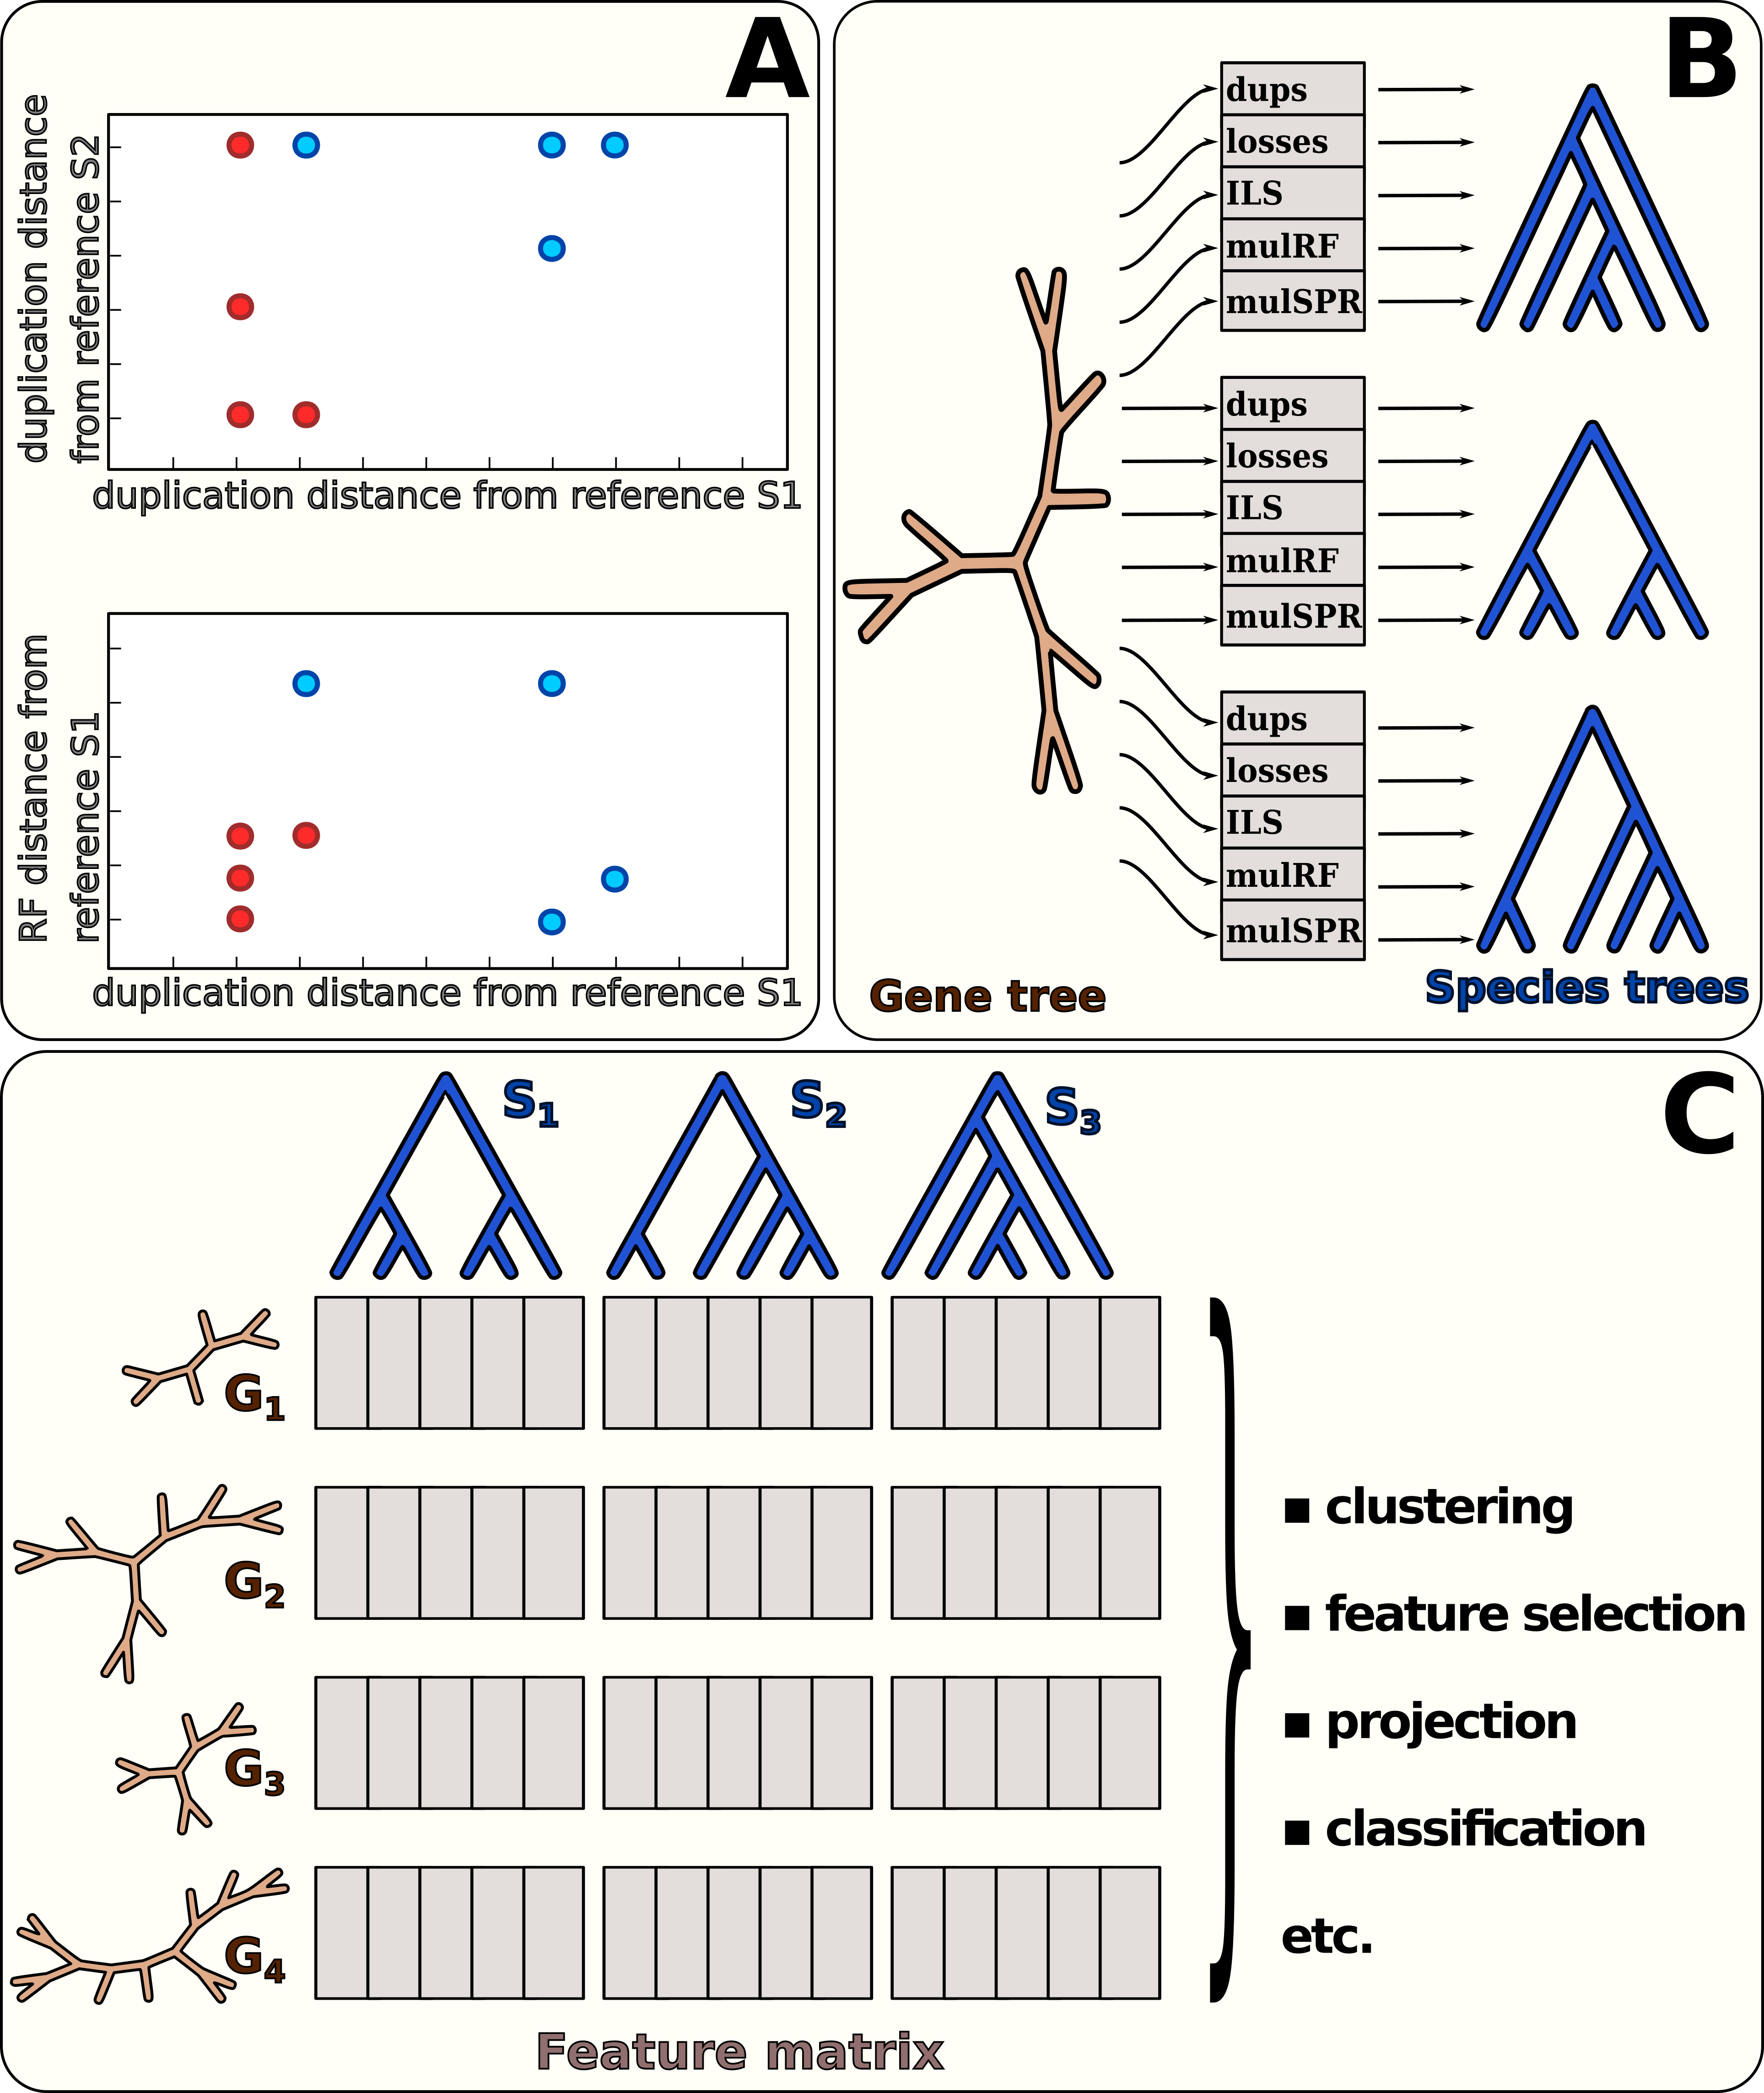
\includegraphics[width = 6in]{figure001.png}\end{minipage}
\caption{\label{figure01}
Schematic representation of the tree signal calculation. In panel A we show two simple cases for a sample of 8 gene
family trees: at the top we compare each gene tree to two distinct reference (species) trees using the minimum number of
duplications (duplication distance), and at the bottom we compare all sample gene trees to a single reference tree, but
using two distinct metrics --- the Robinson-Foulds (RF) distance and the duplication distance. Both comparisons provide
little information in isolation, but when combined allow for distinguishing the two groups of gene families (represented
by distinct colours). Panel B shows how the tree signal of a single gene family tree can be calculated, given a set of
species trees and a set of distances. Notice that currently we work with unrooted gene trees and rooted species trees.
In panel C we show that once we have the tree signal from each gene family, then we can create a feature matrix (‘design
matrix’) which can be used in downstream analyses.
}\end{figure}



\section{Methods}
The gene family trees represent orthogroups or root HOGs <ref>, that is, a tree describing all sequences assumed to
share a common ancestral sequence (including paralogs, or several individuals from the same population). These trees are
the input to the algorithm and may have been estimated by any phylogenetic method --- the algorithm is agnostic to the
source of disagreement (and therefore to the reason for the multiple leaves with same species label) or to the inference
procedure. The reference trees represent possible species trees, and must be on the same set of all species (i.e. all
species must be present in all reference trees). The set of reference trees should capture the variability between gene
trees with respect to the set of distances used to describe them. Therefore a good choice would be a set of optimal
species trees for the most dissimilar sets of gene families, although here we usually limit ourselves to a few species
trees inferred from a single set of gene families, with further randomisation in a few cases. It is important to notice
that the reference species trees are not restricted to the optimal ones (under some notion of optimality) and do not
need to include all optimal species trees. However having good candidates for the species trees will help interpreting
the gene trees in terms of them. The gene trees are assumed to be unrooted since the basic phylogenetic inference models
can’t infer the root location, but our method can be easily adapted for rooted gene family trees. The reference species
trees are rooted, although some distances disregard this information. The reference species trees are fixed beforehand,
but once they are set they can be used to create the “tree signal” of any gene family online, as long as all species
present in the gene family are represented in the reference species trees.

\red{describe the vector}
\begin{equation}
v(t_j,T) = \{d_i(t_j, T) \forall T \in T, i=\left(dups, loss, ils, RF, SPR\right) \} \forall j=1\dots k
\end{equation}


i.e. the spectral signature of gene tree $t_j$ is the set of combinations of distances i and reference trees T in a
specific order. In the simplest case, a single distance and a single tree could be used, as e.g. their RF distance to a
point estimate of their species tree. This would lead to a one-dimensional spectral signature, which may not be able to
discriminate well different gene trees. A natural extension is then to use more reference trees, in such a way that gene
trees now can be closer to one reference or another, or to use more distances, that will describe distinct ways in which
the gene trees relate to the reference.

\subsection{Distances}
We implemented several gene-species tree distances, in particular the reconciliation-based ones available in <guenomu>,
the multi-labelled tree version of the Robinson-Foulds distance called mulRF <citation>, and  two new distances based on
the the same ‘extended’ species tree from the mulRF distance, namely mulSPR and mulHdist. All distances utilise the
topological information only, neglecting branch lengths. Although we refer to them as ‘distances’ they are in fact
dissimilarity measures, and not true distance metrics since they do not satisfy the symmetry condition. The three
reconciliation-based distances implemented are the minimum number of duplications, minimum number of losses, and minimum
number of deep coalescences (also called ancestral polymorphisms or incomplete lineage sortings), and are based on the
LCA mapping between gene tree and species tree nodes. Since they originally work on rooted gene trees, we try all
possible gene rootings and store the minimal distance among all possibilities --- the species tree is rooted, however.

The other three distances are based on the concept of an ‘extended’ species tree, which replaces each leaf from the
species tree by a multifurcation with all leaves from the gene family tree mapping to this species (leaf) <citation>.
The resulting extended species tree and the gene family tree will have thus a one-to-one mapping between leaves. The
mulRF distance is then just the (unrooted) Robinson-Foulds distance between these trees. The mulSPR and the mulHdist,
equivalently, are just the SPR and Hdist distances between the gene family tree and the extended species tree: the SPR
distance is the approximation described in <citation>, and the Hdist is the total cost of matching each edge from the
gene tree to its optimal counterpart on the species tree (it has its name since we use the Hungarian method for solving
this assignment problem). This matching is also used by the SPR algorithm to find the smallest disagreement split
<citation>. The Hdist represents therefore the minimum number of leaves in disagreement per edge, summed over all edges.
If the gene tree is not multi-labelled (i.e. all leaves map to distinct leaves on the species tree) then the mulSPR and
the mulHdist correspond to the SPR and Hdist distances implemented in <citation>. These distances neglect the species
tree root location, treating it as unrooted.

\subsection{Normalisation}
Since we are comparing gene family trees with different numbers of leaves, species, and leaves per species, we must
rescale the distances to a common range. For all implemented distances, lower and upper bounds can be found, but in
practice they are too permissive and therefore we resort to randomisation to find tight bounds for the distances. This
is achieved by, for each gene family t and set of reference species trees T, after calculating the distances $d_i(t, T)$
for all distances i and species trees T, generate a new set of random species trees $\tau$ and calculate the distances to
these trees. We implemented two independent normalisations, that are concatenated into the vector of tree signals: the
p-value distance and the MinMax rescaled distance. The ‘p-value’ distance $p_i(t,T)$ counts the fraction of species trees
in total (i.e. amongst both randomised $\tau$ and reference T) presented a distance as small as the observed:

\begin{equation}
p_i(t,T) = \sum_{\tau and T} I (d_i(t,k) \leq d_i{t,T)) / |\tau and T|
\end{equation}

The MinMax distance $m_i(t,T)$ is the original distance rescaled to the zero-one interval:
\begin{equation}
m_i(t,T) = ( d_i(t,T) - Min ) / (Max - Min)
\end{equation}
where min and max are, respectively, the minimum and maximum distances observed among both $d_i(t,T)$ and $d_i(t,\tau)$.

The vector is thus
\begin{equation}
v(t_j,T) = \{\{p_i(t_j, T), m_i(t_j,T)\}  \forall T\in T, i=\left(dups, loss, ils, RF, SPR\right) \} forall j=1\dots k
\end{equation}

\subsection{Choice of reference trees}
Once the distances (dissimilarity measures in fact) and the reference trees are defined, we can calculate the signature
of each gene tree independently. The more distances are used the more we may discriminate between the gene trees, and
therefore we can implement and use as many measures as possible --- remembering that there are just a few that can be used
in general for a gene tree/species tree pair. However the choice of the reference trees may affect our ability to
distinguish between gene trees, since our rationale is that gene trees can be compared in terms of the species trees
they support according to each biological phenomenon. Given N species, the number of possible rooted reference trees is
r(N)=(2N-3)\!\!, which already exceeds $10^7$ even for N=10. However, in practice we don’t need that many reference trees
since many of them will not be supported by any gene tree in the sample. Ideally our set of reference trees is then all
species trees that can be supported by at least one gene tree in the sample. That is, if there is a distance measure i
and gene tree t  s.t. $d_i(t,T’) < \epsilon(i,t)$ then T’ should be added to the list of reference trees (where
$\epsilon(i,t)$ is a
small, arbitrary value in the distribution of distances $d_i$ over all possible species trees given t). Since finding such
trees T’ can challenging as well, a good strategy seems to be to find trees that summarise the information from subsets
of genes from the sample. One example is to use methods that incorporate uncertainty and therefore output sets of
species trees instead of finding a single point estimate (De Oliveira Martins, Mallo, and Posada 2016). Notice that even
random trees might be at distinct distances from two given gene trees, but this distinction depends also on the
discriminatory power of the distance measure. Also, we expect that by using collections of gene trees in the reference
tree search instead of each gene tree we reduce the number of possible species trees, since small, incomplete gene trees
are not informative in the sense that they favour equally a large number of species trees (not necessarily close to
other gene trees).

Notice that this relies on knowing the set of gene trees in advance, which somehow weakens our argument for continuous
update, but in practice we hope that a broad choice of reference trees (by using not only the ‘optimal’ ones) can
alleviate this problem. <needs rephrasing>


\section{Results}
We tested this model using two simulation scenarios and one real data set. The simulations include both
uniquely-labelled trees, to allow for comparison with traditional pairwise distance-based methods, as well as
genome-level simulation scenarios, leading to mul-trees.

For the first simulation scenario, starting from a random tree T0 on n leaves, we applied a series of consecutive SPR
branch swapping, storing all resulting trees  ${Ti} (0 \leq i leq N)$.  
As a result we know that Ti  and Ti-1 disagree by only
one SPR, Ti  and Ti-2 by two SPRs, etc., neglecting cases where the branch swappings cancel each other out. Therefore we
can use their relative location in this series (the ‘SPR chain’) as an indicator of their dissimilarity. We collected
them into 4 sets of 10 consecutive trees each to serve as our sample gene trees, separated by <y> trees – some of which
were used as reference trees. To test the effect of missing data we randomly removed leaves from each sample tree, such
that trees belonging to the same ‘group’ (i.e. consecutives in our chain of trees) have the same leaves removed. Only
the sample trees have missing leaves, but not the reference trees (by design of our model). [ Both the sample trees
(representing gene trees) and the reference trees (representing species trees) belong to the chain, but only the sample
trees have missing leaves. ]

The results are shown in figure 2, where we compare the effect of using reference trees belonging to the SPR chain (i.e.
similar to the sample trees in an SPR sense) or using randomly selected reference trees on the metric multidimensional
scaling (MDS) projection of the trees. We can conclude that choosing carefully the reference trees (i.e. that are close
to the samples) can help separating the sample gene family trees, even when these sample trees have missing data. On the
other hand using random trees did not seem to compromise the overall separation between groups. In this simulation
scenario all gene tree pairs can be directly compared since we do not have mul-trees (each species is uniquely
represented in the gene family tree), and therefore can be compared using distance matrix-based models (Gori et al.
2016). We therefore used our library to emulate the behaviour of treeCL (Gori et al. 2016) but using the approximate SPR
distance in addition to the RF distance, normalised to account for the unequal number of leaf comparisons. Pairwise
distance matrices creating using both measures provided MDS coordinates comparable to our tree signal using good
reference trees (results not shown). 


\begin{figure}[!htbp]
\begin{minipage}{7in}\centering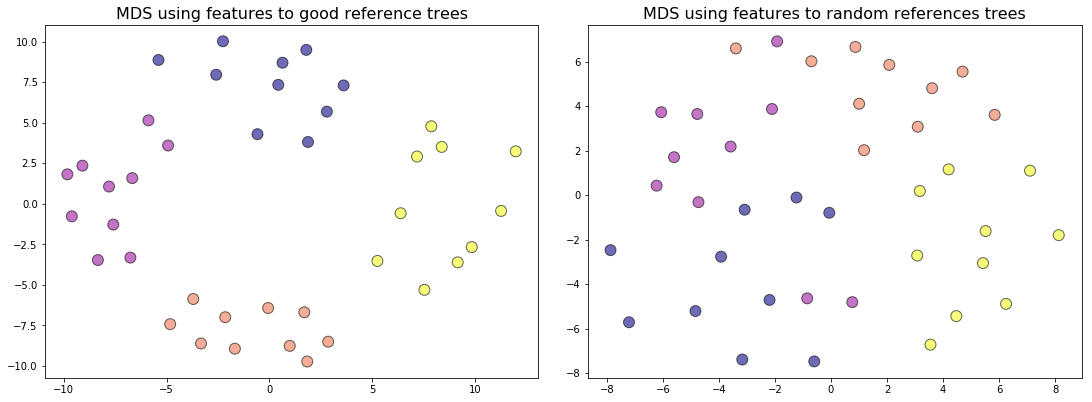
\includegraphics[width = 6.5in]{figure002.png}\end{minipage}
\caption{\label{figure002}
 SPR chain simulation with missing data. On the left panel we see the MDS projections of the samples when their signal
 is calculated from similar reference trees, and on the right we have the projections when random species trees are
 used. The colors represent the four groupings (consecutive trees in the SPR chain, separated from each other by more
 SPR branch swappings) defined in the simulation. 
}\end{figure}


The second simulation scenario was based on a genome-level simulation, where the gene trees are simulated , using the
software Simphy (Mallo, de Oliveira Martins, and Posada 2015), according to the multispecies coalescent within a locus
tree, which is generated under a duplication-loss model from a species tree. We generated 4 species trees with 20
species and from each species tree we simulated 50 gene families, assuming randomly between one or two genomes from each
species (simulating the sampling process of populations under the coalescent). Finally we removed up to half the leaves
from each gene family, and we used 116 trees similar to the true species trees as reference trees --- generated by random
branch swapping on the original ones.

There are many parameters controlling Simphy (from the multispecies coalescent to the birth-death process), and for most
of them we let the software sample from distributions, in order to allow for heterogeneity between gene families. We
tried several such combinations and show here a typical case, based on the observed distribution of leaves and species
per gene family tree, and where a bit less than half the species are common to gene family pairs. The parameters chosen
led to an expectation of one duplication and one loss per branch of the species tree, with 0.2 expected horizontal gene
transfers per branch, and moderate levels of incomplete lineage sorting. Parameter values more extreme led to large gene
families with less than half the species represented, and with very few (less than four) species in common per pair.

The result for a typical simulation is shown in figure 3, where we see that gene families from distinct species trees
can be discriminated.


\begin{figure}[!htbp]
\begin{minipage}{7in}\centering
  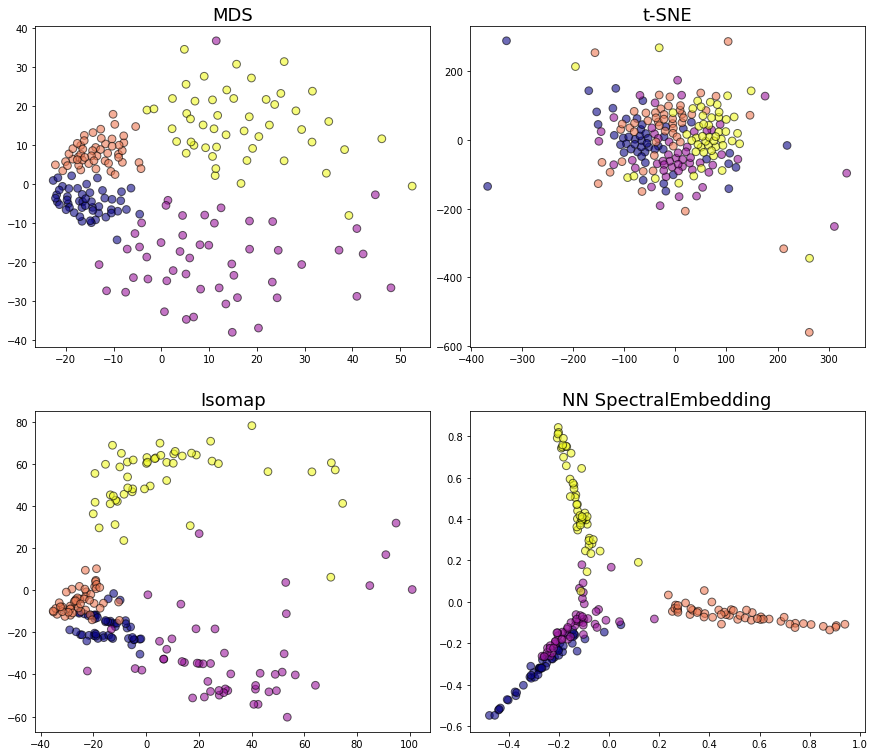
\includegraphics[width = 6in]{figure003a.png}
  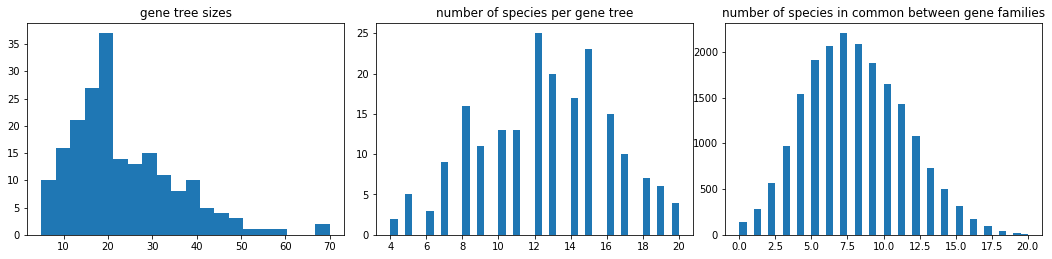
\includegraphics[width = 6in]{figure003b.png}
\end{minipage}
\caption{\label{figure003}
Typical case (simphy simulation). Colors represent underlying species trees.
}\end{figure}

\begin{figure}[!htbp]
\begin{minipage}{7in}\centering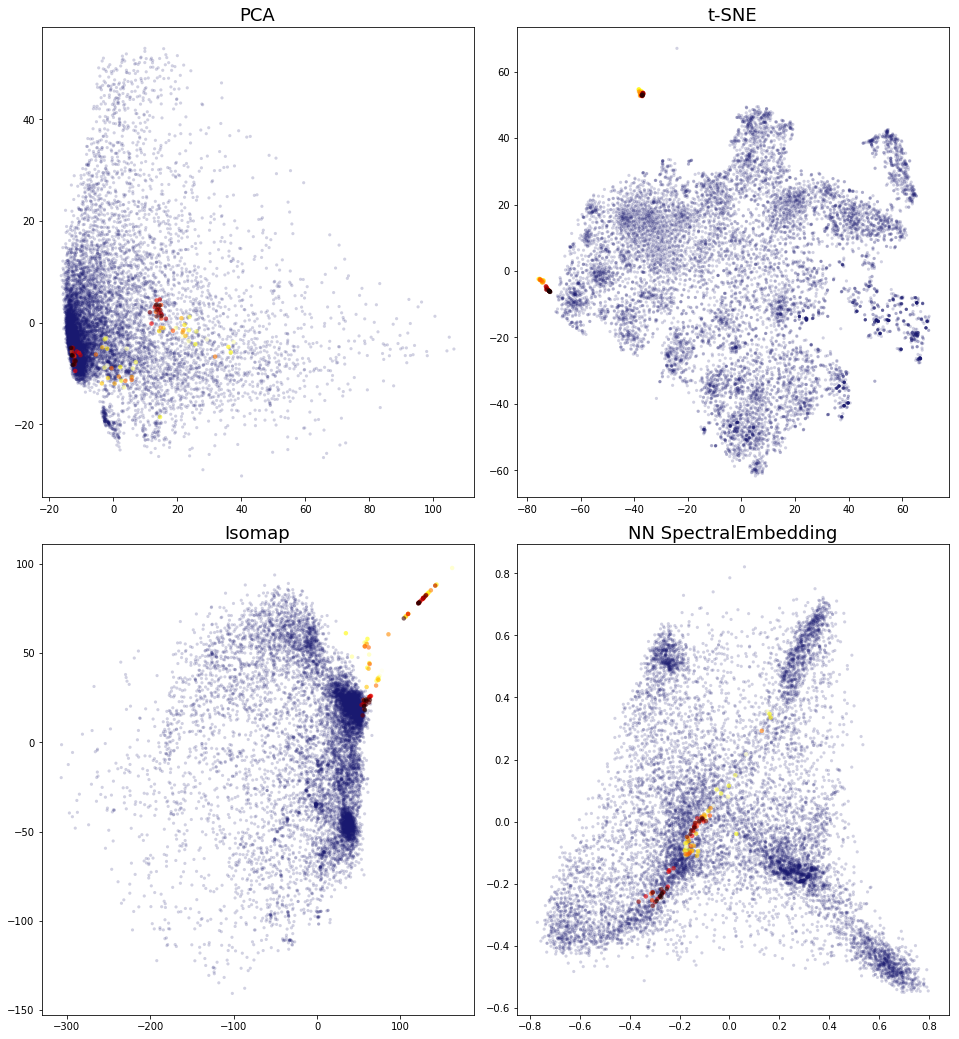
\includegraphics[width = 6.5in]{figure004.png}\end{minipage}
\caption{\label{figure004}
Fungal data set
}\end{figure}




\begin{spacing}{0.8} \bibliography{references} \end{spacing}
\end{document}
